\documentclass[12pt]{article}

\usepackage{prilab}
\usepackage{url}


\begin{document}

\maketitle{Lab 06: Link Analysis}

\section{}

Implement a function that takes as input a graph of hiperlinked documents and
computes the PageRank vector for all documents.

The input graph is a dictionary, where each key is a document ID $d_i$ and each
value is a \texttt{set} containing the documents that \textbf{link to} document
$d_i$. The output is a dictionary where each key is a document ID $d_i$ and
each value is the PageRank value of document $d_i$.

The function should also take as input the number of iterations to perform and
the \emph{damping factor}.

\begin{quote}
    \textbf{Note:} To compute PageRank you also need to know how many outlinks
    a given document has. This value should also be available to the function.
\end{quote}

\section{}

The file \texttt{pri\_cfc.txt} is composed of several text documents from
the CFC collection\footnote{\url{http://www.dcc.ufmg.br/irbook/cfc.html}}. It
contains one document per line, and the first word of each line is the
document ID.

The file \texttt{pri\_links.txt} contains a graph of links between the
documents in the CFC collection. Each line contains
a set of document IDs, where the first ID is a document $d_i$ and the remaining
are the documents \textbf{linked by} $d_i$.

Using this file, compute the PageRank of all documents in the CFC
collection. Print all document IDs and their respective PageRank values, sorted
descending by PageRank value.

You should experimentally determine how many iterations are necessary for the
algorithm to converge.

\begin{quote}
    \textbf{Note:} To compute PageRank of a document $d$, you need to know
    which documents link to $d$. Thus, you need to invert the given link graph.
\end{quote}

\section{}

Using the Whoosh search engine from a previous lesson, implement a script that performs
searches and returns the results ordered by a combination of textual similarity
and PageRank. Use any formula you want to combine both values.

The following example code shows how to perform a query using Whoosh and obtain
the textual similarity score:
\begin{verbatim}
from whoosh.index import open_dir
from whoosh.qparser import *
ix = open_dir("indexdir")
with ix.searcher() as searcher:
    query = QueryParser("content", ix.schema, group=OrGroup).parse(u"first document")
    results = searcher.search(query, limit=100)
    for i,r in enumerate(results):
        print r, results.score(i)
\end{verbatim}

\section{Pen and Paper Exercise}

Consider the following graph, representing a set of Web pages.
\begin{center}
    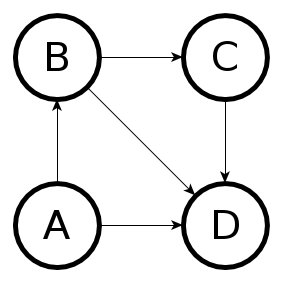
\includegraphics[scale=.5]{graph01}
\end{center}

\begin{enumerate}
\item Compute the PageRank value for each page. Assume a damping factor of
    $0.1$.
\item Compute the hub and authority values of each page, using the HITS algorithm.
\end{enumerate}
\end{document}

%%% Local Variables: 
%%% mode: latex
%%% TeX-master: t
%%% End: 

